\documentclass[xcolor={dvipsnames}, handout]{beamer}
%\documentclass[xcolor={dvipsnames}]{beamer}
%\usepackage{amsmath,amsfonts,amssymb,pxfonts,eulervm,xspace}
\usepackage{amsmath, amsfonts, amssymb, mathtools, eulervm, xspace}
\usepackage{bm}
\usepackage{mathrsfs} % math script fonts
\usepackage{tikz}
\newtheorem{prop}{Proposition} %math?

\usetikzlibrary{cd} % commutative diagrams
\usepackage{subcaption} % subfigure float captioning

\usepackage{tabulary}
\usepackage{tabularx}
\usepackage{booktabs}
\usepackage{multirow}

\usepackage{graphicx}

\usepackage{appendixnumberbeamer} 
\usepackage{comment}
\usepackage{minted}
\setminted[python]{fontsize=\scriptsize, 
                   linenos,
                   numbersep=8pt,
                   autogobble, 
                   frame=lines,
                   bgcolor=bg,
                   framesep=3mm} 
\usepackage{notation} % move this later

\graphicspath{.figures/}

\usepackage[backend=bibtex, style=alphabetic, sorting=none, doi=false,isbn=false,url=false, giveninits=true]{biblatex}
\bibliography{../draft/glasslab_viz.bib}

\usetheme{ccnycrest}

\newenvironment{changemargin}[2]{%
\begin{list}{}{%
\setlength{\topsep}{0pt}%
\setlength{\leftmargin}{#1}%
\setlength{\rightmargin}{#2}%
\setlength{\listparindent}{\parindent}%
\setlength{\itemindent}{\parindent}%
\setleng{}th{\parsep}{\parskip}%
}%
\item[]}{\end{list}}

\begin{document}

\title{Topological Equivariant Artist Model}

\begin{frame}
	\titlepage
    Hannah Aizenman\\
    Advisor: Dr. Michael Grossberg \\
    Committee: Dr. Robert Haralick, Dr. Lev Manovich, Dr. Huy Vo\\
    External Member: Dr. Marcus Hanwell
\end{frame}
\section{Introduction}

\begin{frame}{Visualizations are structure preserving maps}
    %add arrow between data and vizualizations
    % we're focused on building good arrows 
    \begin{figure}
        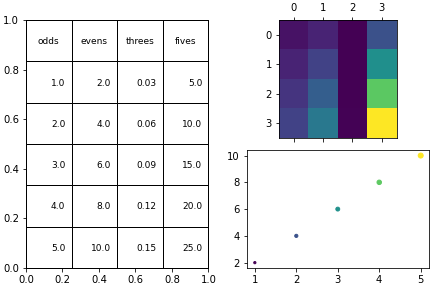
\includegraphics[width=\textwidth]{figures/intro/viz_same.png}
    \end{figure}
    \pause 
    \begin{description}
        \item[equivariance] properties of data and visual encoding match
    \pause 
        \item[continuity] connectivity of data and visual encoding match
    \end{description}
\end{frame}

\begin{frame}{Domain specific libraries assume data structure\cite{HeerSoftware2006}}
    \begin{table}
        %\renewcommand{\arraystretch}{2}
        \begin{tabulary}{\textwidth}{|L|l|l|}\toprule
            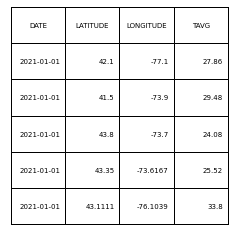
\includegraphics[width=.24\textwidth]{figures/intro/table.png} & 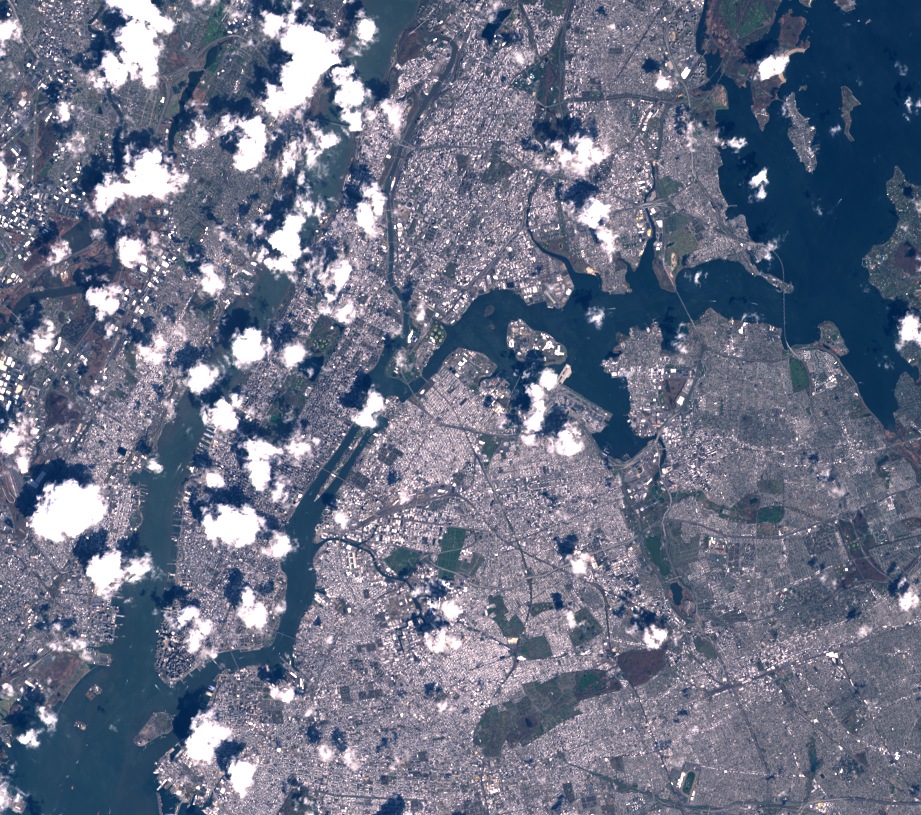
\includegraphics[width=.3\textwidth]{figures/intro/landsat.png} & 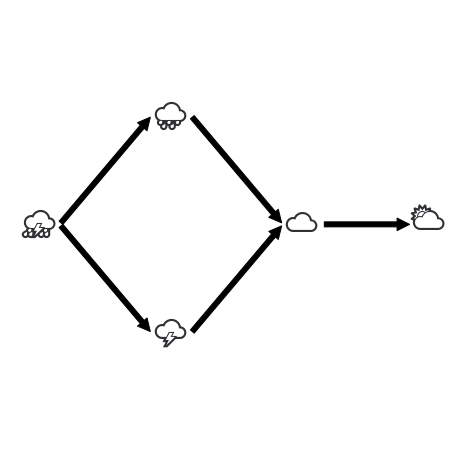
\includegraphics[width=.33\textwidth]{figures/math/graph.png} \\
            ggplot\cite{wickhamGgplot2ElegantGraphics2016a}  & ImageJ\cite{schneiderNIHImageImageJ2012}& Gephi\cite{bastianGephiOpenSource2009}\\
            Vega\cite{satyanarayanDeclarativeInteractionDesign2014} & ImagePlot\cite{studiesCulturevisImageplot2021} & Graphviz\cite{ellsonGraphvizOpenSource2002}\\
            Altair\cite{vanderplasAltairInteractiveStatistical2018}& Napari\cite{nicholas_sofroniew_2021_4533308} & Networkx\cite{HagbergExploringNetwork2008}\\
             Tableau\cite{StoltePolaris2002,hanrahanVizQL2006,MackinlayShowme2007} & &\\
             \bottomrule
        \end{tabulary}
    \end{table}
\end{frame}


\begin{frame}{General purpose libraries can't\cite{toryRethinkingVisualizationHighlevel2004}}
    \begin{figure}
        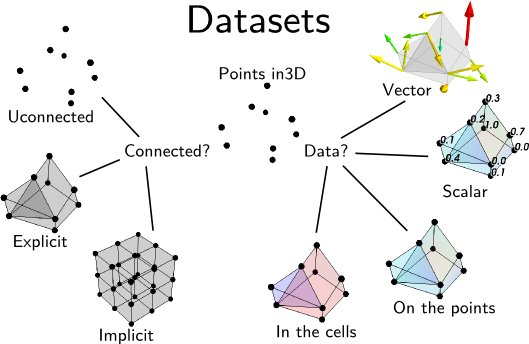
\includegraphics[height=.5\textheight]{figures/intro/dataset_diagram.png}
        \caption{Data Representation, MayaVi 4.7.2 docs\cite{DataRepresentationMayavi}}
    \end{figure}
    \begin{enumerate}
        \item Matplotlib\cite{hunterMatplotlib2DGraphics2007} $\rightarrow$Seaborn\cite{waskom2020seaborn}, xarray \cite{hoyer2017xarray} 
        \item D3 \cite{bostockDataDrivenDocuments2011}
        \item VTK \cite{hanwellVisualizationToolkitVTK2015,geveci2012vtk}(MayaVi\cite{RamachandranMayaVI2011})$\rightarrow$ Titan\cite{brianwylieUnifiedToolkitInformation2009}, ParaView\cite{ahrens2005paraview}
    \end{enumerate}
\end{frame}

\begin{frame}{Best practices in visualization design}
    \begin{description}
        \item[Expressiveness] structure preserving mappings\cite{mackinlayAutomatingDesignGraphical1986}
        \pause
        \item[Graphical Integrity] graphs show \textbf{only} the data\cite{tufteVisualDisplayQuantitative2001}
        \pause 
        \item[Naturalness] easier to understand when properties match\cite{norman_things_smart}
    \end{description}
\end{frame}

\subsection{Contributions}
\begin{frame}{Contributions}
    \begin{description}
        \item[Topological] continuity  
        \item[Equivariant] monoid action 
        \item[Artist] Matplotlib $\textit{artist}: \textit{data} \rightarrow \textit{graphic}$ 
        \item [Model] 
    \end{description}
\end{frame}


\section{Mathematical Framework}

\begin{frame}{Topological Equivariant Artist Model}
    \centering
    An artist $\mathscr{\vartist}$ is an equivariant map 
    \begin{equation*}\huge
        \mathscr{\vartist}: \mathscr{\dtotal} \rightarrow \mathscr{\gtotal}
    \end{equation*}
    from data $\mathscr{\dtotal}$ space to graphic $\mathscr{\gtotal}$ space. 
\end{frame}


\subsection{Data Model}
\begin{frame}{Model data as a fiber bundle \cite{butlerVectorBundleClassesForm1992,butlerVisualizationModelBased1989}}
    A fiber bundle is a tuple $(\dtotal,\,\dbase,\,\pi ,\,\dfiber)$ defined by the map $\pi$
    \begin{equation*}
        \label{eq:fiber_bundle}
        \begin{tikzcd}[ampersand replacement=\&]
            \dfiber \arrow[r, hook] \& \dtotal \arrow[r, "\pi"] \& \dbase
        \end{tikzcd}
    \end{equation*}
    \begin{description}
        \pause
        \item[total space \dtotal] topology
        \pause
        \item[fiber space \dfiber] schema
        \pause
        \item[base space \dbase] continuity
    \end{description}
\end{frame}

\begin{frame}{Encode variable types in a schema like fiber \cite{spivakDatabasesAreCategories2010,spivakSIMPLICIALDATABASES}}
    \begin{figure}[H]
        \centering
        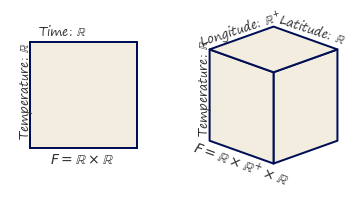
\includegraphics[width=\textwidth]{figures/math/fiber.png}
    \label{fig:data_fiber_example}
    \end{figure}
\end{frame}

\begin{frame}{Structure of components of \dfiber}
    \begin{figure}[H]
        \centering
        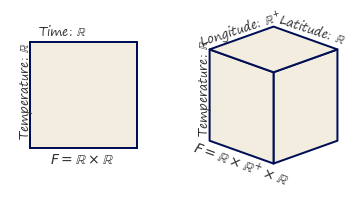
\includegraphics[height=.3\textheight]{figures/math/fiber.png}
    \label{fig:data_fiber_example}
    \end{figure}
        \begin{equation*}
            \dfiber = \dfiber_0 \times \ldots \times \dfiber_i \times \ldots \times \dfiber_n
        \end{equation*}
        \pause
        Monoid actions $\monoid_{i}$ (e.g. rotation, partial ordering) define the structure on $\dfiber_i$
        \begin{equation*}
            \bullet: \monoid_i\times \dfiber_i \rightarrow \dfiber_i
        \end{equation*}
        where $\bullet$ is associative and has an identity action. 
\end{frame}


\begin{frame}{\dbase\ is an indexing space}
    \begin{figure}[H]
        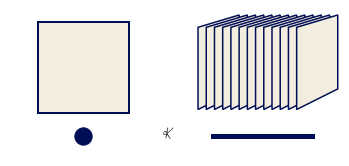
\includegraphics[width=1\textwidth]{figures/math/base.png}
    \label{fig:base_example}
    \end{figure}
\end{frame}

\begin{frame}{Structural \textit{keys} with associated \textit{values} \cite{munznerVisualizationAnalysisDesign2014}}
\begin{figure}
    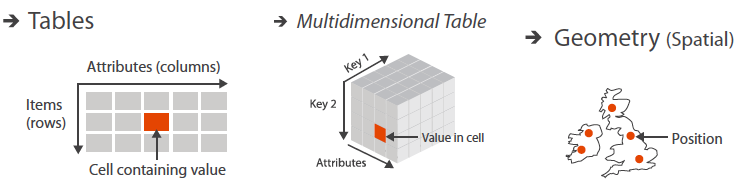
\includegraphics[width=1\textwidth]{figures/intro/munzner_datatypes.png}
    \caption{Figure 2.8 in Munzner's Visualization Analysis and Design\cite{munznerVisualizationAnalysisDesign2014}}
\end{figure}
\pause
\begin{figure}[H]
    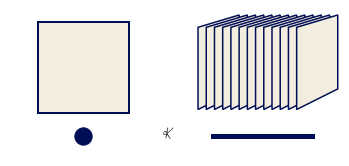
\includegraphics[width=.5\textheight]{figures/math/base.png}
    \label{fig:base_example}
\end{figure}
\end{frame}


\begin{frame}{Data are sections \dsection\ on \dtotal}
    For any fiber bundle, there exists a map
    \begin{equation*}
        \begin{tikzcd}[ampersand replacement=\&]
            \dfiber \arrow[r, hook] \& \dtotal \arrow[d, "\pi"'] \\
                              \& \dbase \arrow[u, "\dsection"', bend right]
        \end{tikzcd}
    \end{equation*}
     s.t. $\pi(\dsection(\dbasepoint)) = \dbasepoint$. $\Gamma(\dtotal)$ is the set of all global sections.
     \begin{figure}[H]
        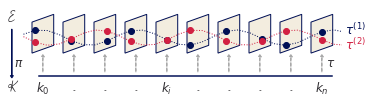
\includegraphics[width=1\linewidth]{figures/math/fiberbundle.png}
        \label{fig:data_sections}
    \end{figure}
\end{frame}


\subsection{Graphics}
\begin{frame}{Graphic Bundle $(\gtotal,\,\gbase,\,\pi ,\,\gfiber)$} % watch dr explaination
    Continuity is preserved via the many \gbasepoint\ to one \dbasepoint\ map $\vindex: \gbase\rightarrow\dbase$
    \begin{equation*} 
        \begin{tikzcd}[ampersand replacement=\&]
            F \arrow[r, hook] \& E \arrow[d, "\pi"']              \& D \arrow[r, hook] \& H \arrow[d, "\pi"']                                 \\
                              \& K \arrow[u, "\tau"', bend right] \&                   \& S \arrow[ll, "\xi"'] \arrow[u, "\rho"', bend right]
            \end{tikzcd}
        \end{equation*}
    \pause
    \gfiber\ is a proxy for the target display, for example $(x,\, y,\, r,\, g,\, b) \in \gfiber$
    \pause
    \begin{figure}[H] %%%bring up one at a time
        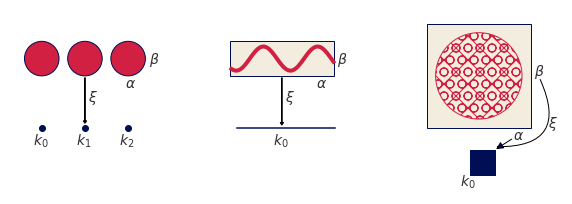
\includegraphics[width=1\textwidth]{figures/math/retraction_maps.png}
        \label{fig:graphic_retraction_map}
    \end{figure}
\end{frame}

\subsection{Artist}
\begin{frame}{Visual bundle $(\vtotal,\,\dbase,\,\pi ,\,\vfiber)$}
    \begin{equation*}
        \mathcal{A}:\mathcal{E}\rightarrow\mathcal{H}
    \end{equation*}
\pause
\begin{equation*}
    \label{eq:artist_diagram}
    \begin{tikzcd}[ampersand replacement=\&]
        \dtotal^{\prime} \arrow[r, "\vchannel"] \arrow[rd, "\pi"'] \& \vtotal \arrow[d, "\pi"] \& \vindex^*\vtotal \arrow[r, "\vmark"] \arrow[d, "\vindex^*\pi"'] \arrow[l, "\vindex^*"'] \& \gtotal \arrow[ld, "\pi"] \\
                                              \& \dbase                  \& \gbase \arrow[l, "\vindex"']                                              \&                    
        \end{tikzcd}
\end{equation*}
\pause
\begin{equation*}
    \vartist: \mathcal{O}(\dtotal) \rightarrow \mathcal{O}(\gtotal)
\end{equation*}
\end{frame}

\begin{frame}{Visualization Assembly Function}
    \begin{figure}
        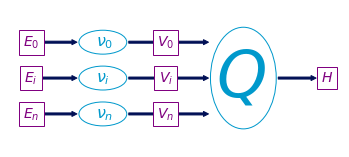
\includegraphics[width=\textwidth]{figures/math/path_of_q.png}
    \end{figure}
    \pause
    \begin{equation*}
        \label{eq:nu_expanded}
        \{\vchannel_{0}, \ldots, \vchannel_{n}\}: \{\dsection_{0}, \ldots, \dsection_{n}\} \mapsto \{\vsection_{0}, \ldots, \vsection_{n}\}
    \end{equation*}
    \pause
    \begin{equation*}
        Q = \nu \circ \tau
    \end{equation*}
\end{frame}


\begin{frame}{Group Equivariance: Stevens' Scales \cite{stevensTheoryScalesMeasurement1946}}
\begin{table}[H]
    \begin{tabularx}{\textwidth}{|l|l|X|}\toprule
        \textbf{scale} & \textbf{group} & \textbf{constraint} \\\midrule
        nominal & permutation &  $\text{if } \delement_1 \neq \delement_2 \text{ then } \vchannel (\delement_1) \neq\vchannel(\delement_2)$\\
        ordinal &  monotonic & $\text{if } \delement_1 \leq \delement_2 \text{ then } \vchannel (\delement_1) \leq \vchannel(\delement_2)$\\
        interval &  translation &  $\vchannel (x + c) = \vchannel(x) + c$ \\
        ratio &  scaling &  $\vchannel(xc) = \vchannel(x)*c $\\ \bottomrule
    \end{tabularx}
\end{table}
\end{frame}

\begin{frame}{Monoid Equivariance: Partial Orders}
    \begin{figure} %break out steps/reveal
        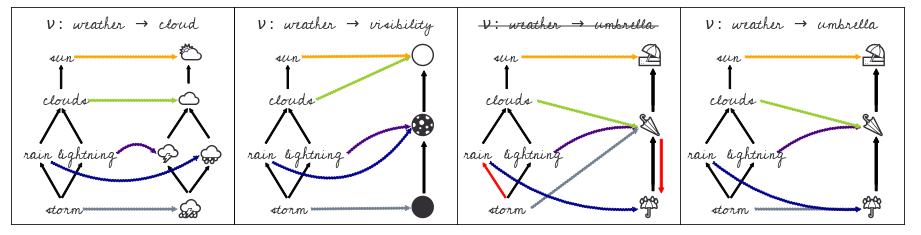
\includegraphics[width=1\textwidth]{figures/math/monoid_equivariant.png}
    \end{figure}
\end{frame}


\begin{frame}{Visualization Equivariance}
    \begin{figure}[H]
        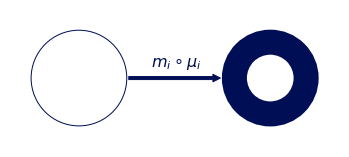
\includegraphics[width=\textwidth]{figures/math/diff_type_q.png}
    \end{figure}
    \begin{equation*}
        \vmark(\vsection) = \vmark(\vsection^{\prime})\implies \vmark(m\circ\vsection) = \vmark(m\circ\vsection^{\prime})
    \end{equation*}
  
\end{frame}

\begin{frame}{Scatter: $\vmark(xpos, ypos)(\alpha, \beta)$}
    \begin{figure}[H]
        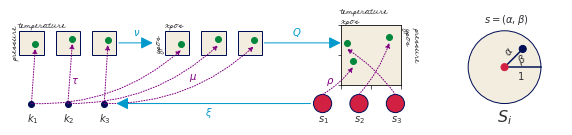
\includegraphics[width=1\textwidth]{figures/math/scatter.png}
    \end{figure}   
\end{frame}

\begin{frame}{Line: $\vmark(xpos, \hat{n_{1}}, ypos, \hat{n_{2}})(\alpha, \beta)$ }
    \begin{figure}[H]
        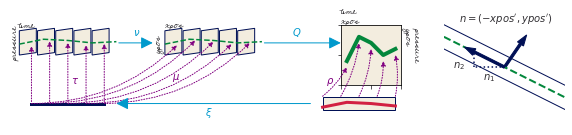
\includegraphics[width=1\textwidth]{figures/math/line.png}
    \end{figure}
\end{frame}

\begin{frame}{Image $\vmark(xpos, ypos, color)$}
    \begin{figure}[H]
        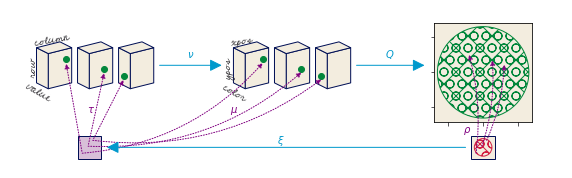
\includegraphics[width=1\textwidth]{figures/math/image.png}
    \end{figure}
\end{frame}

\begin{frame}{Build \vmark\ over \dbase:\vmarkd}
\begin{figure}[H]
    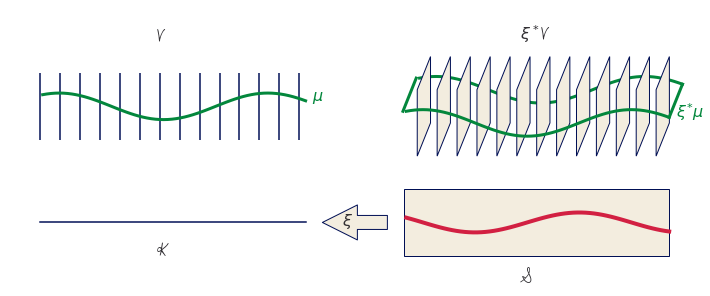
\includegraphics[width=1\textwidth]{figures/math/q_hat.png}
\end{figure}
\begin{equation*}\label{eq:qhat_q_s}
    \vmarkd(\vsection(\dbasepoint))(\gbasepoint) \coloneqq \vmark((\vsectionpull)(\gbasepoint))
\end{equation*} 
\end{frame}

\begin{frame}{Composition of artists $+ \coloneqq \sqcup \dtotal_{i}$} 
    \begin{figure}
        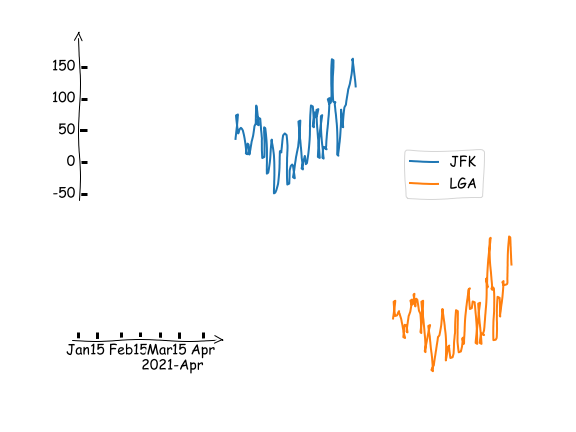
\includegraphics[width=1\textwidth]{figures/math/exploding_artist.png}
    \end{figure}
\end{frame}


\section{Prototype}
\begin{frame}{TEAM driven rearchitecture of Matplotlib}
    \begin{itemize}
        \item complex visualizations
        \pause 
        \item structure preserving maps from data to visual
        \begin{itemize}
            \item data and graphics have equivalent continuity
            \item properties are equivariant under monoid actions
        \end{itemize}  
        \pause
        \item fiber bundles are an abstraction
        \begin{itemize}
            \item topologically complex heterogenous data 
            \item target display spaces
        \end{itemize}
    \end{itemize}
\end{frame}

\begin{frame}[fragile]{How do we make things with this model?}
    \begin{figure}[H]
        \begin{subfigure}{0.49\textwidth}
            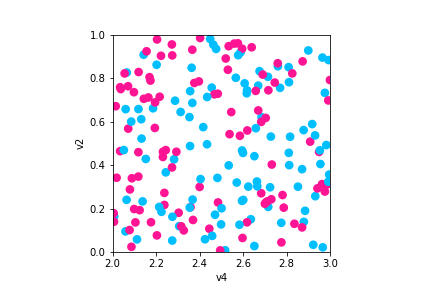
\includegraphics[width=\textwidth]{figures/code/scatter_0.png}
        \end{subfigure}
        \begin{subfigure}{0.49\textwidth}
            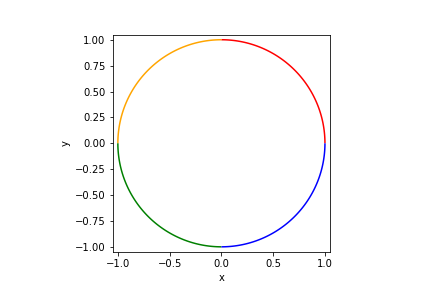
\includegraphics[width=\textwidth]{figures/code/line_1.png}
        \end{subfigure}
    \end{figure}
    \begin{columns}
    \column{0.49\textwidth}
    \begin{minted}{python}
    fig, ax = plt.subplots()
    artist = Point(data, transforms)
    ax.add_artist(artist)
    \end{minted}
    \column{.49\textwidth}
    \begin{minted}{python}
    fig, ax = plt.subplots()
    artist = Line(data, transforms)
    ax.add_artist(artist)
    \end{minted}
    \end{columns}
\end{frame}

\subsection{Visual Transforms}
\begin{frame}[fragile]{How do we implement \vchannel?}
    \begin{minted}{python}
    cmap =  color.Categorical({'true':'deeppink', 'false':'deepskyblue'})
    transforms = {'x': {'name': 'v4', 'encoder': lambda x: x},
                    'y': {'name': 'v2', 'encoder': lambda x: x},
                    'facecolors': {'name':'v3', 'encoder': cmap}, 
                    's':{'name': None , 
                        'encoder': lambda _: itertools.repeat(.02)}}
    \end{minted}
    \begin{itemize}
        \item \mintinline{python}{lambda x: x} is identity \vchannel\
        \item \mintinline{python}|{'name':None}| map into \vfiber\ without corresponding \dsection\
        \item \mintinline{python}{color.Categorical} is custom \vchannel
    \end{itemize}
\end{frame}
    

\subsection{Artist}
\begin{frame}[fragile]{Artist} %% rewrite w/ letters in talk
    \begin{minted}{python}
        class ArtistClass(matplotlib.artist.Artist):
            def __init__(self, E, V, *args, **kwargs):
                # set properties that are specific to the artist
                # stash the input E and V
                super().__init__(*args, **kwargs)
        
            def qhat(self, **args):
                # set the properties of the graphic
        
            def draw(self, renderer):
                # returns tau, indexed on fiber then key 
                tau = self.E.view(self.axes) 
                # visual channel encoding applied fiberwise 
                visual = {p_i: nu_i(tau_i)
                          for p_i, nu_i, tau)i 
                          in zip(self.V, tau)}
                self.qhat(**visual)
                # pass configurations off to the renderer
                super().draw(renderer)
        \end{minted}
\end{frame}

\begin{frame}[fragile]{Artists: Scatter \& Line \vmarkd}
\begin{minted}{python}
    class Point(mcollections.Collection):
        def assemble(self, x, y, s, facecolors='C0' ):
            # construct geometries of the circle glyphs in visual coordinates
            # set attributes of glyphs

    class Line(mcollections.LineCollection):
        def assemble(self, x, y, color='C0'):
            # assemble line marks as set of segments 
    \end{minted}
\end{frame}

\subsection{Data}
\begin{frame}[fragile]{Continuity}
    \begin{minted}{python}
class PointData: 
    # Fiberbundle is consistent across all sections
    FB = FiberBundle({'tables': ['vertex']},  
        {'v1': float, 'v2': str, 'v3': float})
    def tau(self, k):
        return # tau evaluated at one point k

class LineData: 
    FB = FiberBundle({'tables': ['edge']},
                {'x' : float, 'y':  float, 'color':mtypes.Color()})
    def tau(self, k): 
        return # tau evaluated on interval k
    \end{minted}
\end{frame}

\begin{frame}[fragile]{Same Artist, Different Data Configurations}
    \begin{figure}[H]
        \begin{subfigure}{0.49\textwidth}
            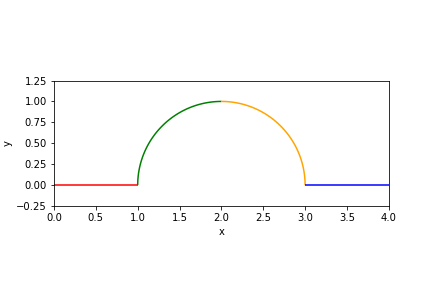
\includegraphics[width=\textwidth]{figures/code/linec_1.png}
        \end{subfigure}
        \begin{subfigure}{0.49\textwidth}
            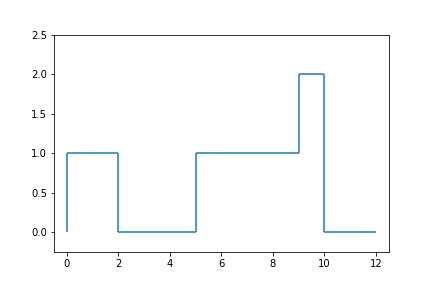
\includegraphics[width=\textwidth]{figures/code/lined_1.png}
        \end{subfigure}
    \end{figure}
\begin{minted}{python}
LineData(FB, edge_table, vertex_table, connect=True)
LineData(FB, edge_table, vertex_table, num_samples=2, connect=False)
\end{minted}
\end{frame}

\begin{frame}{Proposed Work}
\begin{figure}
    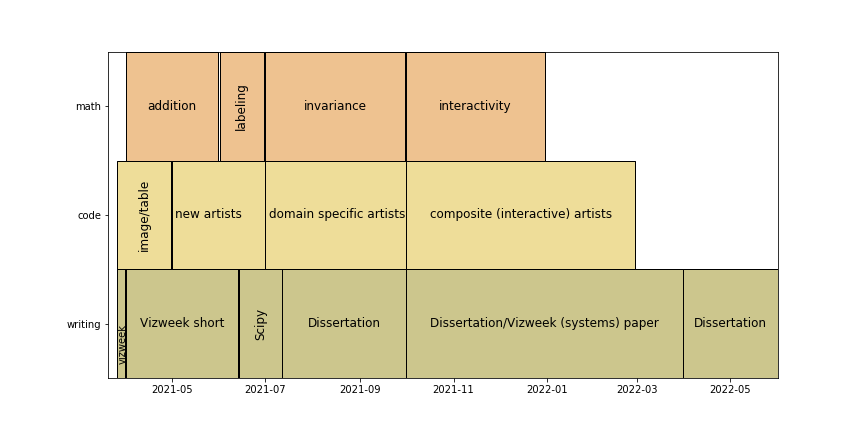
\includegraphics[width=1\textwidth]{figures/intro/gantt.png}
\end{figure}
\end{frame}

\section{References}
\begin{frame}[allowframebreaks]{References}
\printbibliography
\end{frame}
\appendix 

\subsection{Appendix}

\begin{frame}{Mathematical Models of Vizualization}
    \begin{description}
        \item[algebraic process] data and viz transforms are symmetric \cite{kindlmannAlgebraicProcessVisualization2014}
        \begin{equation*}
            \begin{tikzcd}[ampersand replacement=\&]
                \dtotal \arrow[d, "m"'] \arrow[r, "\nu"] \& \vtotal \arrow[r, "Q"]  \& \gtotal \arrow[d, "\varphi(m)"] \\
                \dtotal \arrow[r, "\nu"']                     \& \vtotal \arrow[r, "Q"'] \& \gtotal                  
            \end{tikzcd}
        \end{equation*}
      
        \item[language] APT and GoG: syntax, semantics, and grammar\\ 
        \cite{mackinlayAutomatingDesignGraphical1986,mackinlayAUTOMATICDESIGNGRAPHICAL1987,wilkinsonGrammarGraphics2005}
        \item[functional dependencies] relationship between components \cite{sugibuchiFramwork2009}
        \item[category theory]  \textit{understanding} = \textit{read} $\circ$ \textit{render} \cite{vickersUnderstandingVisualizationFormal2013}    
    \end{description}
\end{frame}

\begin{frame}{Fiber is all possible values a variable can be \cite{spivakDatabasesAreCategories2010,spivakSIMPLICIALDATABASES}}
    Given a space of all possible values \ftotal\
    \begin{equation*}
        \label{eq:data_types}
        \begin{tikzcd}[ampersand replacement=\&]
            \fttype \arrow[r] \arrow[d, "\pi_{\fsection}"'] \& \ftotal \arrow[d, "\pi"] \\
            \fnames \arrow[r, "\fsection"']                  \& \ftypes       
        \end{tikzcd}
    \end{equation*}
    a fiber component is the restricted space $\ftotal_{\fsection(\fname)}$. 
    \begin{equation*}
        \dfiber = \ftotal_{\fsection(\fname)} = \ftotal_{\ftype} 
    \end{equation*}
    \begin{description}
        \item[\ftypes] data types of the variables in the dataset 
        \item[\ftotal] disjoint union of all values of type $\ftype \in \ftypes$ 
        \item[\fnames] variable names, $\fname \in \fnames$
        \item[\fttype] \ftotal\ restricted to the data type of a named variable   
    \end{description}
\end{frame}

\begin{frame}{Monoid actions}
    A monoid \monoid\ is a set with
    \begin{description}
        \item[associative binary operator] $\ast:\monoid \times \monoid\rightarrow \monoid$
        \item[identity element] $e\in \monoid$ such that $e\ast a= a \ast e = a$ for all $a \in \monoid$. 
    \end{description}
    \begin{block}{left monoid action}
    A set \dfiber\ with an action\cite{nlab:action} $\bullet: \monoid\times \dfiber \rightarrow \dfiber$ with the properties:
        \begin{align*}
            \textbf{associativity}\;& \text{for all } f,g \in \monoid \text{ and } x\in \dfiber,\, f\bullet(g\bullet x) = (f\ast g) \bullet x\\
            \textbf{identity}\;& \text{for all } x\in \dfiber, e\in \monoid,\,  e\bullet x = x 
        \end{align*}
    \end{block}
\end{frame}

\begin{frame}{Keeping track of sections with sheafs}
    Restriction maps of a sheaf describe how local $\iota^*\dsection$ can be glued into larger sections \cite{ghristElementaryAppliedTopology2014,ghristHomologicalAlgebraData2018}
    \begin{equation*}
        \label{eq:sheaf}
        \begin{tikzcd}[ampersand replacement=\&]
            \iota^*\dtotal \arrow[d, "\pi"'] \arrow[r, "\iota^*", hook]             \& \dtotal \arrow[d, "\pi"']                  \\
            U \arrow[r, "\iota", hook] \arrow[u, "\iota^{*}\dsection"', bend right] \& \dbase \arrow[u, "\dsection"', bend right]
        \end{tikzcd}
    \end{equation*}
    The inclusion map $\iota: U \rightarrow \dbase$ pulls \dtotal\ over $U$ such that the pulled back $\iota^*\dsection$ only contains records over $U \subset \dbase$.
\end{frame}

\begin{frame}{Rendering: Define a Pixel}
    \begin{columns}
        \column{0.5\textwidth}
        Given a pixel
        \begin{equation*}
        p=\left[y_{top}, y_{bottom}, x_{right}, x_{left}\right]
        \end{equation*}
        the inverse map of the bounding box 
        \begin{equation*}
        \gbase_{p} ={\gsection_{xy}}^{-1}(p)
        \end{equation*}
        is a region $\gbase_p \subset \gbase$ such that 
        \begin{align}
            \scriptstyle r_p &= \scriptstyle \iint\limits_{S_p} \rho_r(s)ds^{2}\\
            \scriptstyle g_p &= \scriptstyle \iint\limits_{S_p} \rho_g(s)ds^{2}\\
            \scriptstyle  b_p &= \scriptstyle \iint\limits_{S_p} \rho_b(s)ds^{2}
        \end{align}
        yields the color of the pixel. 
        \column{0.5\textwidth}
        \begin{figure}[H]
            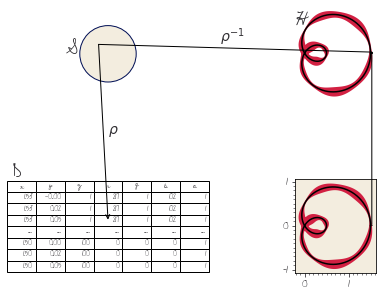
\includegraphics[width=\textwidth]{figures/math/render.png}
        \end{figure}
    \end{columns}
\end{frame}

\begin{frame}{$\mathcal{A}:\mathcal{E}\rightarrow\mathcal{E}$}
    The topological artist is a sheaf map
    \begin{equation*}
    \vartist: \mathcal{O}(\dtotal) \rightarrow \mathcal{O}(\gtotal)
    \end{equation*}
    that carries homomorphism of monoid actions $\varphi: \monoid \rightarrow \monoid^{\prime}$ 
    \cite{cegarraCohomologyMonoidsOperators2019} 
    \begin{equation*}
    \vartist(m\cdot \delement) = \varphi(m)\cdot \vartist(\delement) 
    \end{equation*}
\end{frame}

\begin{frame}{Visual Channel Encoders}
    We define the visual transformers \vchannel\ on components of the data bundle $\dsection_{i}$
    \begin{equation*}
        \label{eq:nu_expanded}
        \{\vchannel_{0}, \ldots, \vchannel_{n}\}: \{\dsection_{0}, \ldots, \dsection_{n}\} \mapsto \{\vsection_{0}, \ldots, \vsection_{n}\}
    \end{equation*}
    as the set of equivariant maps with the constraint 
    \begin{equation*}
        \vchannel_i(m_{\delement}(\dtotal_i)) = \varphi(m_{\delement})(\vchannel_i(\dtotal_i))
    \end{equation*} 
    where $\varphi:\monoid\rightarrow \monoid^{\prime}$ carries a homomorphism of monoid actions. 
\end{frame}

\begin{frame}{\vfiber\ Components}    
\begin{table}[H]
    \renewcommand{\arraystretch}{2}
    \begin{tabulary}{\textwidth}{|l|L|l|}\hline
     $\bm{\vchannel_{i}}$                      & $\bm{\vsection_{i}}$                                                            & $\bm{codomain(\vchannel_{i}) \subset \vfiber_{i}}$  \\ \hline                                              
    position                    & x, y, z, theta, r                                                          & $\mathbb{R}$   \\ \hline
    size                        & linewidth, markersize                                            & $\mathbb{R}^{+}$   \\ \hline
    shape                       & markerstyle                                                      & $\{f_{0}, \ldots, f_{n}\}$ \\ \hline
    color                       & color, facecolor, markerfacecolor, edgecolor  & $\mathbb{R}^{4}$ \\ \hline
    \multirow{2}{*}{texture}    & hatch                                                            & $\mathbb{N}^{10}$\\\cline{2-3}
                                & linestyle                                                        & $(\mathbb{R}, \mathbb{R^+}^{n, n\%2=0})$ \\ \hline              
    \end{tabulary}
    \label{tab:mpl_visual_variable_fiber}
\end{table}
\end{frame}

\begin{frame}{Glyph}
    The glyph is the graphic generated by $\vmark(\gbase_{\dbasepathpoint})$ where the path connected components $\dbasepath \subset \dbase$ are defined 
    \begin{equation*}
    \dbasepath = \{\dbasepathpoint \in \dbase \text{ s. t. } \exists \gamma \text{ s.t. } \gamma(0)=\dbasepoint \text{ and }\gamma(1)=\dbasepathpoint\}
    \end{equation*}
    such that the  path $\gamma$ from \dbasepoint\ to \dbasepathpoint\ is a continuous function from the interval [0,1] and $\gbase_{\dbasepathpoint}$ is the region
    \begin{equation*}
        \begin{tikzcd}[ampersand replacement=\&]
            \gtotal \arrow[r, shift left] \& \gbase_\dbasepathpoint \arrow[rr, "\vindex(\gbasepoint)", shift left] \arrow[l, "\gsection(\gbase_\dbasepathpoint)"] \& \& \dbasepath_{\dbasepoint} \arrow[ll, "\vindex^{-1}(\dbasepath)"]
            \end{tikzcd}
        \label{eq:mark}
    \end{equation*}
    such that the glyph is differentiable, in keeping with Ziemkiewicz and Kosara's description of a glyph\cite{ziemkiewiczEmbeddingInformationVisualization2009}.
\end{frame}

\begin{frame}{Artist Equivalance class}
    When artists share a base space 
    \begin{equation*}
        \dbase_2 \hookrightarrow \dbase_1
    \end{equation*}
    a composition operator can be defined such that the the artists can be considered to be acting on different components of the same section. 
\end{frame}

\begin{frame}[fragile]{Complex \vchannel}
    \begin{minted}{python}
    class Categorical:
        def __init__(self, mapping):
            # check that the conversion is to valid colors
            assert(mcolors.is_color_like(color) for color in mapping.values())
            self._mapping = mapping
    
        def __call__(self, value):
            # convert value to a color
            return [mcolors.to_rgba(self._mapping[v]) for v in values]
    \end{minted}
    That we can test for action equivariance
    \begin{minted}{python}
    def test_nominal(values, encoder):
        m1 = list(zip(values, encoder(values)))
        random.shuffle(values)
        m2 = list(zip(values, encoder(values)))
        assert sorted(m1) == sorted(m2)
    \end{minted}
\end{frame}

\begin{frame}[fragile]{Artist}
    \begin{minted}{python}
        class ArtistClass(matplotlib.artist.Artist):
            def __init__(self, data, transforms, *args, **kwargs):
                # properties that are specific to the graphic
                self.data = data 
                self.transforms = transforms
                super().__init__(*args, **kwargs)
        
            def assemble(self, **args):
                # set the properties of the graphic
        
            def draw(self, renderer):
                # returns K, indexed on fiber then key 
                view = self.data.view(self.axes) 
                # visual channel encoding applied fiberwise 
                visual = {p: t['encoder'](view[t['name']])
                          for p, t in self.transforms.items()}
                self.assemble(**visual)
                # pass configurations off to the renderer
                super().draw(renderer)
        \end{minted}
\end{frame}


\begin{frame}[fragile]{Artists: Scatter \& Line}
\begin{minted}{python}
class Point(mcollections.Collection):
    def assemble(self, x, y, s, facecolors='C0' ):
        # construct geometries of the circle glyphs in visual coordinates
        self._paths = [mpath.Path.circle(center=(xi,yi), radius=si) 
                    for (xi, yi, si) in zip(x, y, s)] 
        # set attributes of glyphs, these are vectorized 
        # circles and facecolors are lists of the same size
        self.set_facecolors(facecolors)

class Line(mcollections.LineCollection):
    def assemble(self, x, y, color='C0'):
        #assemble line marks as set of segments 
        segments = [np.vstack((vx, vy)).T for vx, vy in zip(x, y)]
        self.set_segments(segments)
        self.set_color(color)
\end{minted}
\end{frame}


\begin{frame}[fragile]{View}
\begin{minted}{python}
def view(self, axes):
    table = defaultdict(list)
    for k in self.keys:
        table['index'].append(k)
        for (name, value) in zip(self.FB.fiber.keys(), self.tau(k)[1]):
            table[name].append(value)
    return table
\end{minted}
\begin{description}
    \item [\mintinline{python}{VertexSimplex}] (name, value), value is scaler
    \item [\mintinline{python}{EdgeSimplex}]  (name, value), value is [x0, ..., xn]
\end{description}
\end{frame}

\begin{frame}[fragile]{Fiber Bundle}
    \begin{minted}{python}
    @dataclass
    class FiberBundle:
    """
    Attributes
    ----------
    K: {'tables': []}
    F: {variable name: type}
    """
        K: dict 
        F: dict
    \end{minted}
\end{frame}

\begin{frame}[fragile]{GraphLine Data Model}
\begin{minted}{python}
class GraphLine:
    def __init__(self, FB, edge_table, vertex_table, num_samples=1000,
                        connect=False):
        #set args as attributes and generate distance
        if connect: # test connectivity if edges are continuous
            assert edge_table.keys() == self.FB.F.keys()
            assert is_continuous(vertex_table)

    def tau(self, k):
        # evaluates functions defined in edge table
        return(k, (self.edges[c][k](self.distances) 
                        for c in self.FB.F.keys()))

    def view(self, axes):
        # walk the edge_vertex table to return the edge function
        table = defaultdict(list)
        for (i, (start, end)) in sorted(zip(self.ids, self.vertices), 
                                            key=lambda v:v[1][0]):
            table['index'].append(i)
            # same as view for line, returns nested list
            for (name, value) in zip(self.FB.F.keys(), self.tau(i)[1]):
                table[name].append(value)
        return table
\end{minted}
\end{frame}

\end{document}

